\section{Core Equations}


The equations used in this paper are not intended to define consciousness in closed form.

Consciousness is not a conserved quantity, not an additive measure, and not an object measured as a single variable. The expressions presented here are therefore not "equations of consciousness."

What they fix is the effective region in which consciousness can obtain.

That is, they describe the conditions under which a log-referencing state opens, given the fast predictive process, the slow memory-sedimentation process, the speed difference between them, coupling viscosity, and the gradient of the information potential.

\subsection{Speed Differential}


First, the speed difference between the fast and slow layers is written:

\begin{equation}
\Delta v = v_f - v_s
\end{equation}

Here $v_f$ denotes fast, predictive and reactive dynamics, and $v_s$ denotes slow, sedimentary and stabilizing dynamics.

This differential is not merely descriptive; it defines the condition under which cross-scale referencing becomes possible.

The crucial point is that neither $v_f$ nor $v_s$ alone defines consciousness.

What consciousness involves is not their absolute speeds but the difference maintained between them.

In VED terms, complete synchrony is closure — the disappearance of difference. If the difference disappears entirely, both boundary and flow are lost.

The minimal condition for maintaining a conscious state is therefore:

\begin{equation}
\Delta v \neq 0
\end{equation}

This does not mean consciousness requires strong asynchrony at all times.

It means that a finite speed difference — one that neither collapses into complete synchrony nor reaches complete separation — is required.

\subsection{Coupling Viscosity}


The existence of speed difference alone does not establish a conscious state.

If the fast and slow layers are fully separated, log referencing does not occur even though processing runs. Conversely, if coupling is so strong that both layers collapse to the same speed, the boundary for referencing disappears.

This coupling state is expressed through coupling viscosity $\mu$:

\begin{equation}
\mu > 0
\end{equation}

$\mu$ represents the slipperiness or adhesive resistance of coupling between the fast and slow layers.

If $\mu$ is too small, the layers adhere excessively and the speed difference tends to collapse.

If $\mu$ is too large, the layers slip too freely and log referencing tends to fragment.

What consciousness requires is therefore not mere coupling but a viscous regime that can sustain interaction while preserving the speed difference.

\subsection{Internal Delay}


The relation between speed difference and coupling viscosity appears as internal delay or time buffer $\tau$:

\begin{equation}
\tau \propto \frac{\Delta v}{\mu}
\end{equation}

$\tau$ represents the internal delay during which processing sediments into the slow layer and becomes arranged as a referenceable log.

This delay is not a defect.

Rather, it is because delay exists that immediate processing does not vanish as it arises but gains the opportunity to reach the slow layer as a log.

If $\tau$ is too small, processing approximates immediate reaction and lacks referenceable thickness.

If $\tau$ is too large, the correspondence between current processing and log sedimentation breaks and the conscious state fragments.

The conscious state therefore exists in an intermediate region:

\begin{equation}
\tau_{\min} < \tau < \tau_{\max}
\end{equation}

This range is referred to in this paper as the consciousness stability window.

\subsection{Effective Torque}


Next, the quantity through which speed difference appears not merely as delay but as the transformation load for opening referencing is defined.

As introduced in §5.3, this paper calls it the effective torque-like quantity $\mathcal{T}$:

\begin{equation}
\mathcal{T} = \kappa \frac{\Delta v}{\mu}
\end{equation}

Here $\kappa$ is a scale factor.

$\mathcal{T}$ does not represent psychological will or agency.

It represents the structural load required for the speed difference between fast and slow layers to be transformed without rupture.

Torque Converter Attention is the mechanism that transforms this $\mathcal{T}$ into a processable form.

The crucial point is that $\mathcal{T}$ does not eliminate the difference; it is the quantity that makes transmission possible while the difference is preserved.

\subsection{IFGT Coupling}


The expressions so far have treated only speed difference and coupling viscosity.

However, which logs are referenced in a conscious state is not arbitrary.

Which logs are easily referenced, and which processing tends to sediment into the slow layer, is biased by the gradient of the information potential $\Phi$.

The general variables of IFGT are information density $I$, information flow $J$, and information potential $\Phi$.

In this paper they are used as projected variables inside a biological-cognitive observation window. Thus $I$, $J$, and $\Phi$ should not be read as direct identities between consciousness and the general IFGT field, but as effective coordinates for log density, log-referencing flow, and meaning potential.

The basic relations are:

\begin{equation}
\frac{\partial I}{\partial t} + \nabla \cdot J = \sigma
\end{equation}

\begin{equation}
J = -D \nabla I + \mu_I F
\end{equation}

\begin{equation}
F = -\nabla \Phi
\end{equation}

\begin{equation}
\Phi = K * I
\end{equation}

Here $\sigma$ is the generation-dissipation term for information density, $D$ is the diffusion coefficient, $\mu_I$ is the mobility of information flow, and $K$ is the kernel giving the potential from information density.

In the context of this paper, $\Phi$ functions as the potential of meaning or information.

Log referencing is therefore not merely a function of speed difference; it is directed by the meaning gradient.

Including this effect, the effective torque-like quantity is extended to:

\begin{equation}
\mathcal{T}_{\Phi} \sim \kappa \frac{\Delta v}{\mu} \left|\nabla \Phi\right|
\end{equation}

$\mathcal{T}_{\Phi}$ is the effective quantity in which time-scale difference and meaning gradient are coupled.

Even with large speed difference, if the meaning gradient is weak, log referencing has no stable direction.

Conversely, even with a strong meaning gradient, if the speed difference has vanished, no boundary opens for referencing.

What consciousness involves is the coupling of both.

\subsection{Consciousness Window}


Combining the above, the conscious state is expressed as the region satisfying the following conditions:

\begin{equation}
0 < |\Delta v| < \Delta v_{\max}
\end{equation}

\begin{equation}
\mu_{\min} < \mu < \mu_{\max}
\end{equation}

\begin{equation}
\tau_{\min} < \tau < \tau_{\max}
\end{equation}

\begin{equation}
\mathcal{T}_{\min} < \mathcal{T}_{\Phi} < \mathcal{T}_{\max}
\end{equation}

These are not completed expressions for measuring consciousness numerically.

They are conditions constraining the region in which consciousness can obtain.

If speed difference reaches zero, the boundary collapses into synchrony.

If speed difference is too large, referencing ruptures.

If coupling viscosity is too low, the layers fuse.

If coupling viscosity is too high, the layers slip excessively.

If the meaning gradient is too weak, log referencing loses direction.

If the meaning gradient is too strong, referencing becomes over-fixed to specific wells.

Consciousness is therefore not a point but a window.

This window is called in this paper the consciousness window.

Figure~\ref{fig:consciousness-window} shows the consciousness window as a finite non-closure regime.

\begin{figure}[H]
\centering
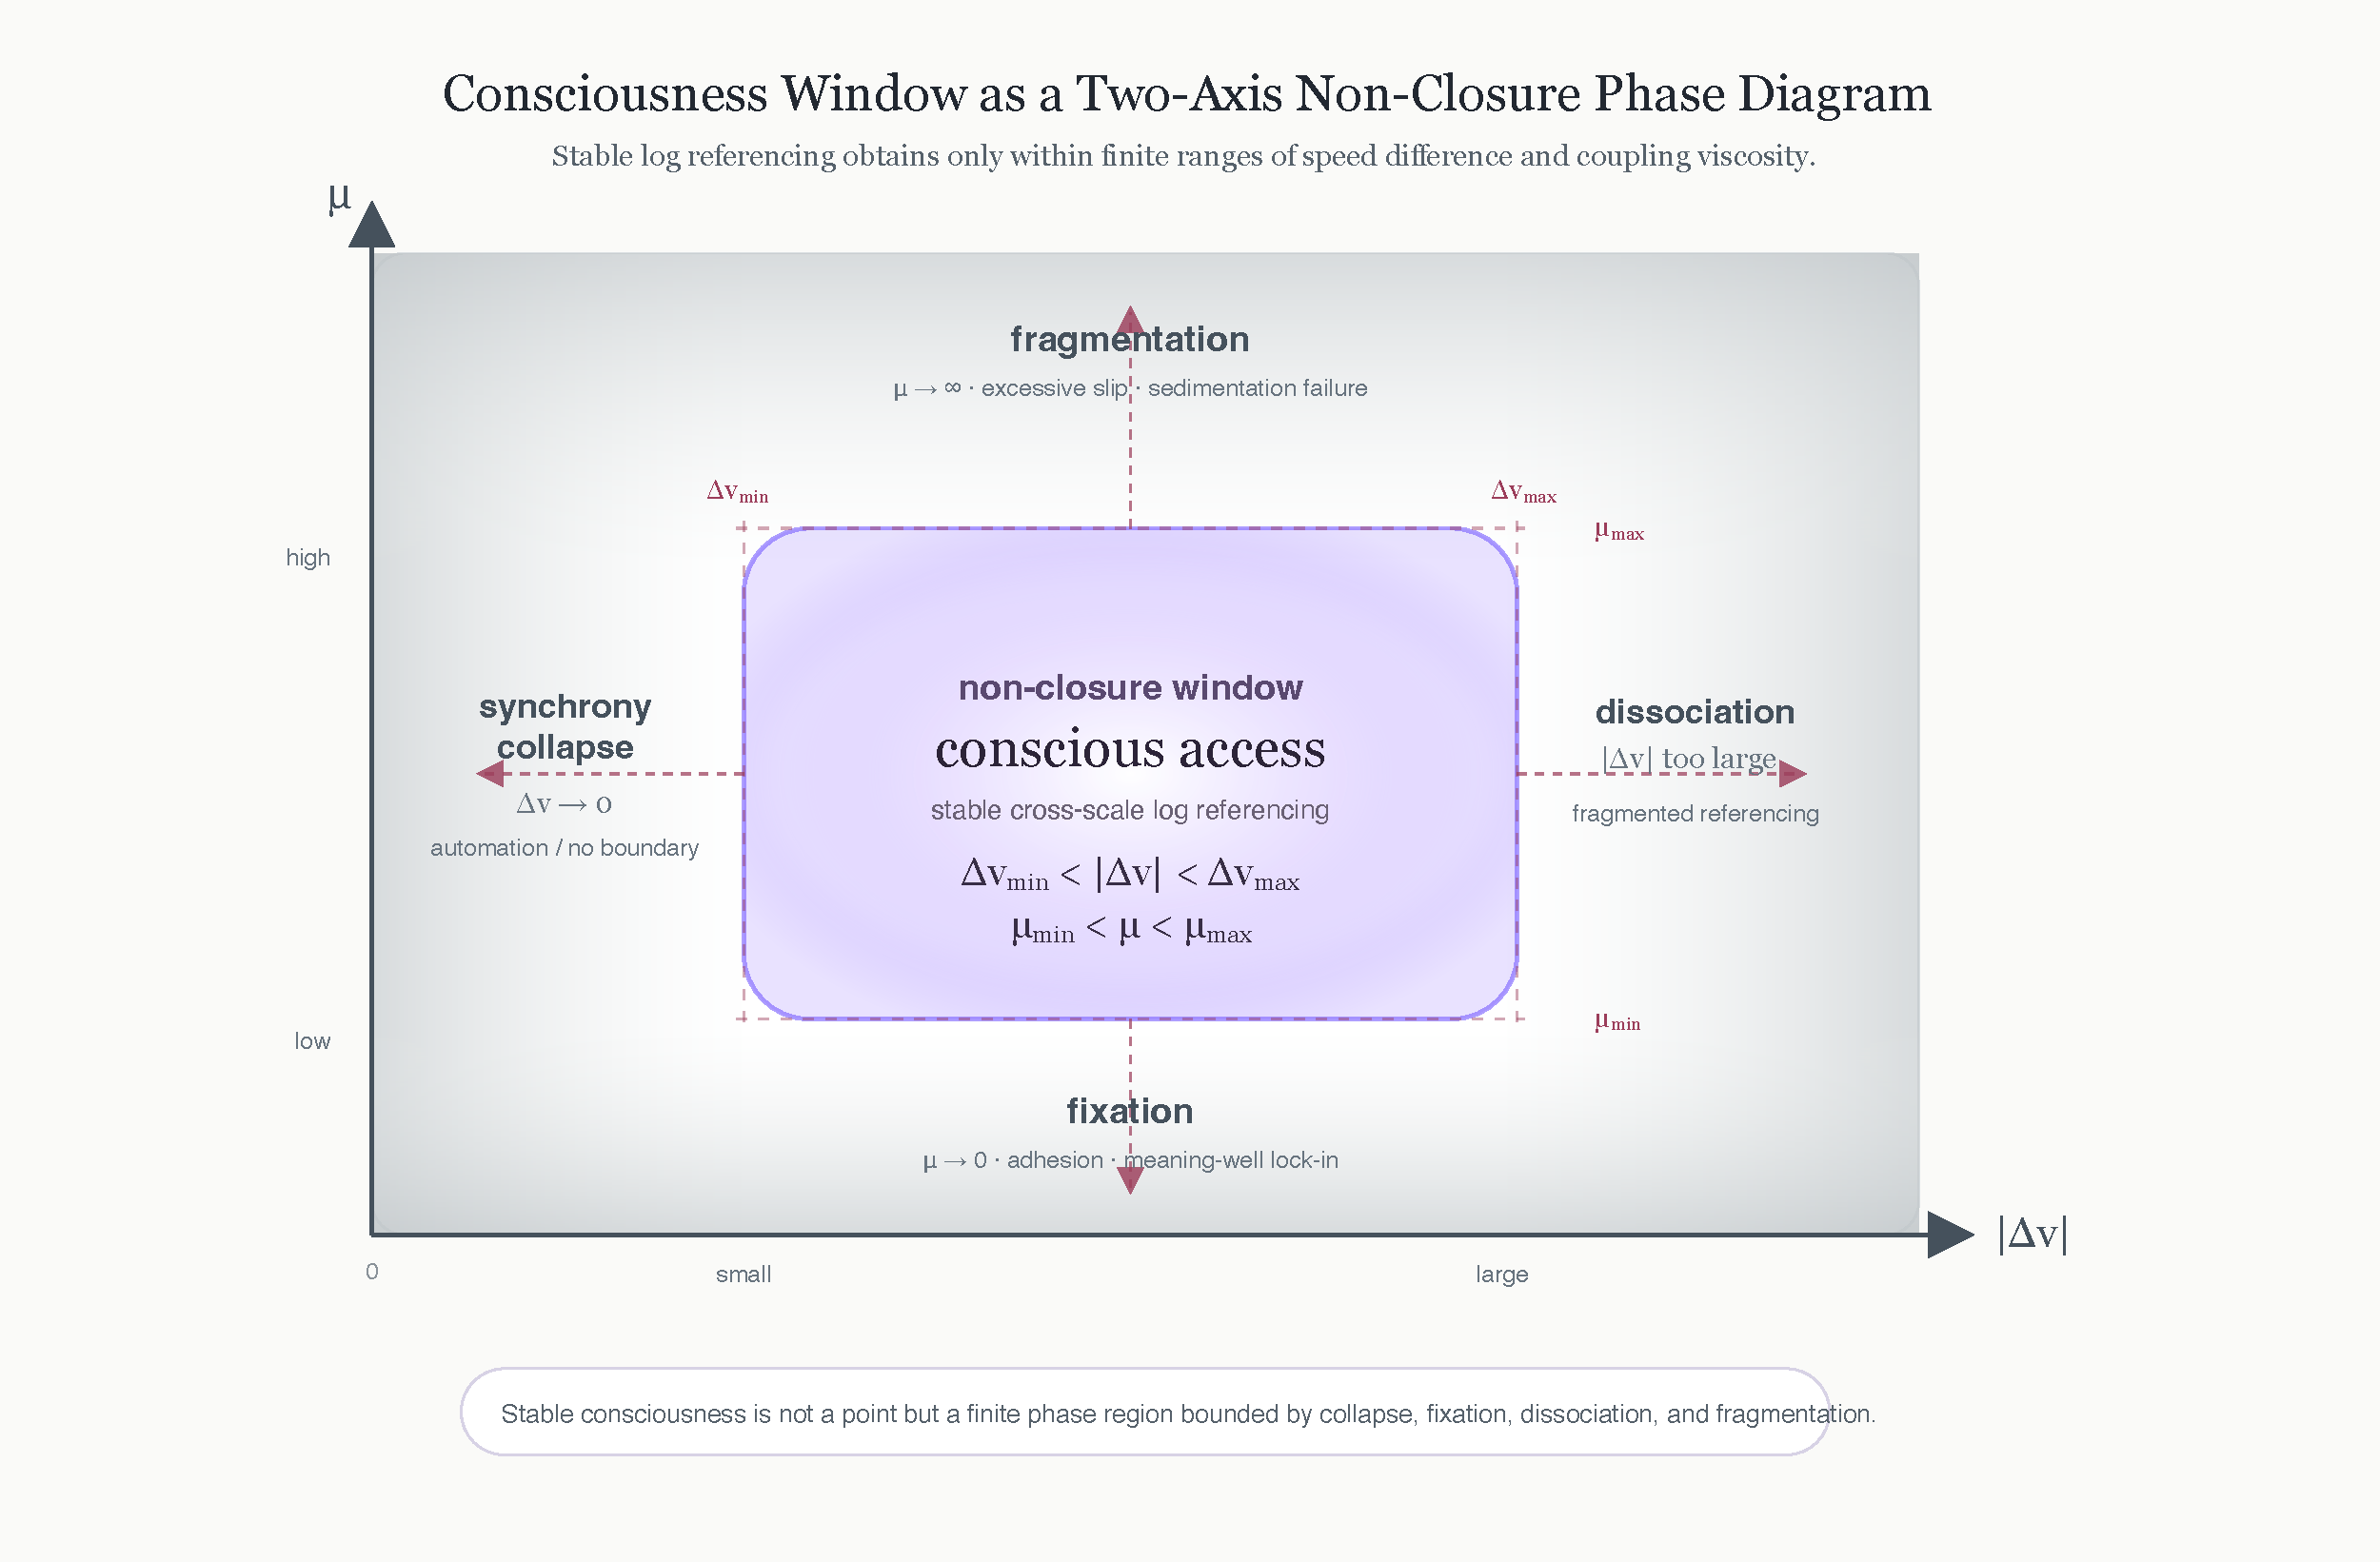
\includegraphics[width=0.86\linewidth]{figures/figure3_nonclosure_window.pdf}
\caption{
Consciousness window as a two-axis non-closure phase diagram.
Stable log referencing obtains only within finite ranges of speed difference and coupling viscosity.
Outside this window, the system tends toward synchrony collapse, dissociation, fragmentation, or fixation.
}
\label{fig:consciousness-window}
\end{figure}

\subsection{Non-Closure Condition}


From the VED perspective, consciousness is maintained not as complete closure but as a state of non-closure.

Complete closure is the boundary representation at which difference vanishes, flow stops, and structure can no longer be maintained as an ordinary generated state.

Consciousness is not such a state.

Consciousness is a dynamic state in which difference persists, flow exists, and maintenance continues within a range that does not rupture.

The minimal condition for consciousness is therefore:

\begin{equation}
\Delta v \neq 0, \qquad \nabla \Phi \neq 0, \qquad \frac{\partial I}{\partial t} \neq 0
\end{equation}

This does not mean consciousness must fluctuate strongly at all times.

It means that complete stasis, complete synchrony, and complete closure are incompatible with the maintenance of a conscious state.

Consciousness is the state in which logs are referenceable within a temporal structure that does not close completely.

In the language of VED, this non-closure condition is equivalently expressed through the closure degree difference $\Delta C = C_s - C_f$ as $0 < \Delta C < \Delta C_{\max}$ (see §6.4 for the full mapping). The two descriptions — speed difference and closure degree difference — are different coordinates on the same structural condition; neither grounds the other.

\subsection{Summary}


The expressions presented in this section do not generate consciousness.

They constrain the conditions under which consciousness can obtain.

The position of this paper, stated minimally:

\begin{equation}
\text{Consciousness} \;\sim\; \text{Log Referencing}\!\left(\Delta v, \mu, \tau, \mathcal{T}_{\Phi}, \nabla \Phi\right)
\end{equation}

More intuitively, consciousness opens under the following conditions:

\begin{itemize}
\item Speed difference exists.
\item Coupling has not broken.
\item Delay is maintained.
\item Meaning gradient exists.
\item Complete closure has not been reached.
\end{itemize}

In this sense, consciousness is not a product.

Consciousness is a log-referencing state that opens when temporal difference, viscosity, meaning gradient, and non-closure simultaneously obtain.
